% 2010 年上海卷理科第 12 题：正方形纸片 ABCD 与对角线交点 O，剪去 △AOB 后沿 OC、OD 折叠。
% 来源 PDF：普通高考/2010/2010上海理.pdf，SHA-256 e6181a8e02bfda976d5a2cee9432881769c184da4d3fca3b5a4d75c57a497ec6。
% 原页：第 1 页（A3 三栏）第 2 栏下部，书页码 627。
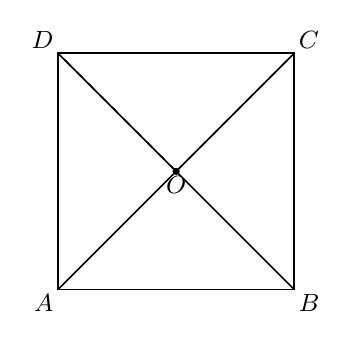
\begin{tikzpicture}[semithick, every node/.style={inner sep=1.4pt, font=\small}]
  \coordinate (A) at (0,0);
  \coordinate (B) at (3,0);
  \coordinate (C) at (3,3);
  \coordinate (D) at (0,3);
  \coordinate (O) at (1.5,1.5);
  \draw (A) -- (B) -- (C) -- (D) -- cycle;
  \draw (A) -- (C);
  \draw (B) -- (D);
  \draw[dashed] (O) -- (C);
  \draw[dashed] (O) -- (D);
  \fill (O) circle (1.3pt);
  \node[below left] at (A) {$A$};
  \node[below right] at (B) {$B$};
  \node[above right] at (C) {$C$};
  \node[above left] at (D) {$D$};
  \node[below] at (O) {$O$};
\end{tikzpicture}
